\documentclass[11pt]{article}

% ---------- Packages ----------
\usepackage[utf8]{inputenc}
\usepackage[T1]{fontenc}
\usepackage[margin=1in]{geometry}
\usepackage{amsmath, amssymb}
\usepackage{booktabs}
\usepackage{array}
\usepackage{enumitem}
\usepackage{xcolor}
\usepackage{tikz}
\usetikzlibrary{shapes.geometric, arrows.meta, positioning, fit, backgrounds}
\usepackage{listings}
\usepackage{hyperref}
\hypersetup{colorlinks=true, linkcolor=blue, urlcolor=blue}

% ---------- TikZ styles ----------
\tikzset{
  block/.style   = {rectangle, draw, rounded corners, align=center,
                     fill=blue!8, minimum height=1cm, minimum width=2.8cm,
                     inner sep=6pt},
  group/.style   = {rectangle, draw, dashed, rounded corners, inner sep=10pt},
  arrow/.style   = {-{Stealth[length=3mm]}, thick},
}

% ---------- Listings style ----------
\definecolor{codebg}{gray}{0.96}
\lstset{
  basicstyle=\ttfamily\small,
  backgroundcolor=\color{codebg},
  frame=single,
  rulecolor=\color{gray!40},
  breaklines=true,
  columns=fullflexible,
  keepspaces=true,
  showstringspaces=false,
  xleftmargin=6pt, xrightmargin=6pt,
  aboveskip=8pt, belowskip=8pt,
}

\title{\textbf{Phase 1 --- Transforms}\\[4pt]
\large Part A: 2D frames, translation, rotation}
\author{Robotics + AI Mentor Notes}
\date{\today}

\begin{document}
\maketitle

\begin{abstract}
\noindent Goal of this phase: understand \textbf{coordinate frames} and how to move
points between them. This is \emph{the} language of robotics --- every joint,
camera, and object has a frame, and a robot's whole job is relating them.
Intuition first, math second, then you implement and verify.
\end{abstract}

\tableofcontents
\bigskip
\hrule

% =====================================================================
\section{Why transforms? (the motivating problem)}

Your robot camera sees a red cube ``40\,cm ahead and 10\,cm to the left
\textbf{of the camera}.'' But the robot arm doesn't move relative to the camera ---
it moves relative to its \textbf{base}. So you must answer:

\begin{quote}
``Where is the cube \textbf{relative to the robot base}?''
\end{quote}

Converting a position from one frame (``as seen by the camera'') to another frame
(``as the base understands it'') is a \textbf{transform}. That's the entire idea.
Master this and robotics stops being mysterious.

% =====================================================================
\section{What is a coordinate frame?}

A \textbf{frame} is just an origin (a chosen zero point) plus axes (directions).
The \emph{same} physical point has \emph{different numbers} in different frames.

\begin{center}
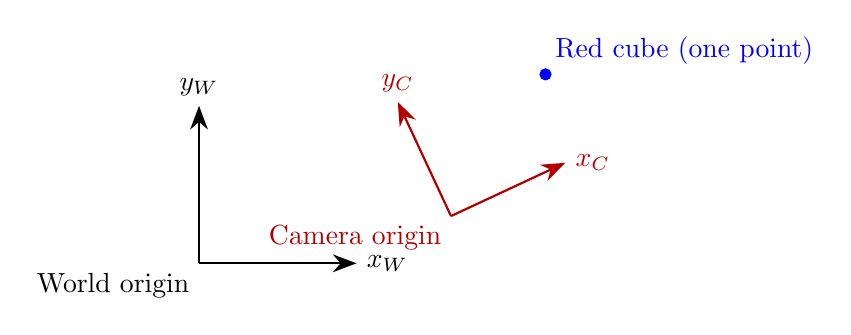
\begin{tikzpicture}
  % world frame
  \draw[arrow] (0,0) -- (2,0) node[right]{$x_W$};
  \draw[arrow] (0,0) -- (0,2) node[above]{$y_W$};
  \node[below left] at (0,0) {World origin};
  % camera frame, translated and rotated
  \begin{scope}[shift={(3.2,0.6)}, rotate=25]
    \draw[arrow, red!70!black] (0,0) -- (1.6,0) node[right]{$x_C$};
    \draw[arrow, red!70!black] (0,0) -- (0,1.6) node[above]{$y_C$};
    \node[red!70!black, below left] at (0,0) {Camera origin};
  \end{scope}
  % the one physical point
  \filldraw[blue] (4.4,2.4) circle (2pt) node[above right, blue]{Red cube (one point)};
\end{tikzpicture}
\end{center}

The cube is one real thing, but:
\begin{itemize}[leftmargin=*]
  \item In the \textbf{camera} frame it might be $(0.40, 0.10)$.
  \item In the \textbf{world} frame it might be $(1.2, 0.5)$.
\end{itemize}

Neither is ``wrong'' --- they're the same point described from different
viewpoints.

\begin{center}
\emph{A point is a vector of numbers; a frame is the context that gives those
numbers meaning.}
\end{center}

% =====================================================================
\section{Points as vectors}

In 2D, a point is just two numbers:
\[
  \mathbf{p} = \begin{bmatrix} x \\ y \end{bmatrix}
\]
Example: \texttt{p = [0.4, 0.1]} means $x=0.4$\,m, $y=0.1$\,m from that frame's
origin.

% =====================================================================
\section{Translation (shifting the origin)}

If frame $B$'s origin sits at position $\mathbf{t} = [t_x, t_y]$ \textbf{within
frame $A$}, then a point known in $B$ is expressed in $A$ by \textbf{adding} the
offset:
\[
  \mathbf{p}_A = \mathbf{p}_B + \mathbf{t}
\]

\textbf{Intuition:} ``start where $B$'s origin is, then walk out to the point.''

Example: camera origin is at $[1.0, 0.0]$ in the world. Cube is $[0.4, 0.1]$ in the
camera frame (pointing the same way). In the world:
\[
  [0.4, 0.1] + [1.0, 0.0] = [1.4, 0.1].
\]

% =====================================================================
\section{Rotation (turning the axes)}

If frame $B$ is \textbf{rotated} by angle $\theta$ relative to frame $A$, a point in
$B$ is expressed in $A$ by multiplying with the \textbf{rotation matrix}:
\[
  R(\theta) = \begin{bmatrix} \cos\theta & -\sin\theta \\ \sin\theta & \cos\theta \end{bmatrix},
  \qquad
  \mathbf{p}_A = R(\theta)\,\mathbf{p}_B
\]

\textbf{Intuition:} rotating a point by $\theta$ swings it counter-clockwise around
the origin. The matrix is just ``the recipe'' that mixes $x$ and $y$ to do that
swing.

\paragraph{Sanity checks (do these in your head):}
\begin{itemize}[leftmargin=*]
  \item $\theta = 0$: $R = \begin{bmatrix}1&0\\0&1\end{bmatrix}$ (identity)
  $\rightarrow$ point unchanged. \checkmark
  \item Rotate $[1, 0]$ by $90^\circ$: expect $[0, 1]$ ($x$-axis swings up to the
  $y$-axis).
\end{itemize}

Worked math for the $90^\circ$ case ($\cos 90^\circ=0,\ \sin 90^\circ=1$):
\[
  \begin{bmatrix}0&-1\\1&0\end{bmatrix}\begin{bmatrix}1\\0\end{bmatrix}
  = \begin{bmatrix}0\\1\end{bmatrix} \quad\checkmark
\]

% =====================================================================
\section{Your task (implement + verify)}

Open \texttt{src/utils/transforms\_2d.py}. It has three functions with
\texttt{TODO}s:

\begin{enumerate}[leftmargin=*]
  \item \texttt{translate(point, offset)} --- add the offset.
  \item \texttt{rotation\_matrix(theta)} --- build $R(\theta)$ (angle in
  \textbf{radians}).
  \item \texttt{rotate(point, theta)} --- apply the rotation matrix to the point.
\end{enumerate}

Then run the file. It has a built-in self-check that prints \textbf{PASS/FAIL} for
each.

\begin{lstlisting}[language=bash]
cd ~/Music/projects_abbas/ROBOT_VLA
python3 src/utils/transforms_2d.py
\end{lstlisting}

\textbf{Expected output when correct:}
\begin{lstlisting}
[test] translate     -> PASS
[test] rotation_matrix -> PASS
[test] rotate 90deg  -> PASS
[test] rotate 0deg   -> PASS
All tests passed.
\end{lstlisting}

\textbf{If you get FAIL:} read which line failed, re-check the formula above, fix,
rerun. Report your output and I'll confirm before we go to Part~B (combining
rotation + translation into a single \textbf{homogeneous transform}, then 3D).

% =====================================================================
\section*{What's next (do NOT start yet)}
\addcontentsline{toc}{section}{What's next}
\begin{itemize}[leftmargin=*]
  \item Part B: homogeneous transforms (rotation + translation in one matrix).
  \item Part C: 3D frames, and the TF tree ROS~2 uses.
\end{itemize}

\end{document}
